% 独自のコマンド

% ■ アブストラクト
%  \begin{jabstract} 〜 \end{jabstract}  :日本語のアブストラクト
%  \begin{eabstract} 〜 \end{eabstract}  :英語のアブストラクト

% ■ 謝辞
%  \begin{acknowledgment} 〜 \end{acknowledgment}

% ■ 文献リスト
%  \begin{bib}[100] 〜 \end{bib}


\newif\ifjapanese

\japanesetrue  % 論文全体を日本語で書く(英語で書くならコメントアウト)

\ifjapanese
  \documentclass[a4j,twoside,openright,11pt]{jreport} % 両面印刷の場合。余白を綴じ側に作って右起こし。
  %\documentclass[a4j,11pt]{jreport}                  % 片面印刷の場合。
  \renewcommand{\bibname}{参考文献}
  \newcommand{\acknowledgmentname}{謝辞}
\else
  \documentclass[a4paper,11pt]{report}
  \newcommand{\acknowledgmentname}{Acknowledgment}
\fi
\usepackage{thesis}
\usepackage{ascmac}
\usepackage{graphicx}
\usepackage{multirow}
\usepackage{url}
\bibliographystyle{jplain}

\bindermode  % バインダー用余白設定

% 日本語情報(必要なら)
\jclass  {修士論文}                             % 論文種別
\jtitle    {近接関係に基づく情報取得システム}    % タイトル。改行する場合は\\を入れる
\juniv    {慶應義塾大学大学院}                  % 大学名
\jfaculty  {政策・メディア研究科}               % 学部、学科
\jauthor  {郡山 隼人}                       % 著者
\jhyear  {26}                                   % 平成○年度
\jsyear  {2014}                                 % 西暦○年度
\jkeyword  {Bluetooth、近接、情報取得、修士論文}     % 論文のキーワード
\jproject{} %プロジェクト名
\jdate{}

% 英語情報(必要なら)
\eclass  {Master's Thesis}                            % 論文種別
\etitle    {Information gathering system based on proximity}      % タイトル。改行する場合は\\を入れる
\euniv  {Keio University}                             % 大学名
\efaculty  {Graduate School of Media and Governance}  % 学部、学科
\eauthor  {Hayato Koriyama}                           % 著者
\eyear  {2014}                                        % 西暦○年度
\ekeyword  {Bluetooth, proximity, Information gathering, Master Thesis}          % 論文のキーワード
\eproject{}                 %プロジェクト名
\edate{}





\begin{document}

\ifjapanese
  \jmaketitle    % 表紙(日本語)
\else
  \emaketitle    % 表紙(英語)
\fi

% ■ アブストラクトの出力 ■
%	◆書式:
%		begin{jabstract}〜end{jabstract}	:日本語のアブストラクト
%		begin{eabstract}〜end{eabstract}	:英語のアブストラクト
%		※ 不要ならばコマンドごと消せば出力されない。



% 日本語のアブストラクト
\begin{jabstract}

モバイルデバイスの進化につれて、
一般的なモバイルデバイスに共通して搭載されているセンサやモジュールは豊富になった。
同時に、それらと組み合わせることで実現されるContext-basedなサービスも一般化している。
これらのサービスはコンテキストに特化した情報の取得を促進させつつも、
情報はサービス内限定の閉鎖的な文脈となることが多い。

対して、近年大きく発展してきたSNSやコミュニケーションサービスは、
Webの持つ自由度を持ったまま進化を続けてきた。
しかし、同じ場所に居合わせた人同士がこのようなサービスの上で情報をやりとりするには
あらかじめユーザが互いの信頼において連絡方法を確立しなくてはならない。
そのため、見知らぬ人同士がデジタルな情報共有まで辿り着くには、壁が存在する。

本論文では、
近接した人同士が状況や場所に関する情報を取得し、共有するためのシステムを提案する。

本システムは、ユーザの近接情報を元にした情報取得と共有を促進させ、
さらにWeb上での閲覧と編集を可能にすることで、コンテキストに対するWebからの情報取得を実現する。
Context-basedなサービスとWebサービスの特性を組み合わせることで、
近接した人同士が情報をやりとりする行為を簡便なものへと発展させつつ、
Context-basedなサービスの閉鎖性を緩和させる。

本論文では、提案するシステムの実装と試用の際の議論から、システムの有効性について考察し、
近接関係に基づく情報取得の展望を示す。


\end{jabstract}



% 英語のアブストラクト
\begin{eabstract}

Through the evolution of mobile devices,
Sensors and modules that are mounted on the general mobile devices was abundant.
At the same time, the Context-based service that is realized by combining them has also been generalized.

Although these services to promote the gathering of information that specializes in context,
this information is often a closed context in the service.

In contrast, in recent years large development to have the SNS and communication services,
It has continued to evolve while holding the degree of freedom with the Web.

However, people with each other, which happened to be the same place to exchange information on such services
Beforehand users must be established how to contact in user's trust.

Therefore, the wall is present to up until arrive at strangers to share users digital information.

In this paper,
We propose a sharing information system for people with in close proximity to each other to obtain information about the situation or location.

This system is to promote the sharing and gathering information
that is based on the proximity of the users.

And by enabling editing and viewing on the Web,
to achieve the information obtained from the Web for the context.

By combining the characteristics of the Context-based services and Web services,
And while developing the users in close proximity
to communicate information to the simple ones,
thereby relieving the closing of the Context-based services.

In this paper,
from the discussion of the implementation and testing of the proposed system,
we consider the effectiveness of the system,
and show the outlook of information gathering system based on proximity.

\end{eabstract}
  % アブストラクト。要独自コマンド、include先参照のこと

\tableofcontents  % 目次
\listoffigures    % 表目次
\listoftables    % 図目次

\pagenumbering{arabic}

\chapter{序論}\label{chap:introduction}

本章では、本論文における研究の動機と目的を述べた後、
本論文の構成について概略を述べる。

\newpage

\section{研究動機}

本論文は、近接情報に基づく情報共有と情報取得のためのアプリケーションを提案し、
その設計および開発について述べ、場所や状況を共有する人々のための情報共有を実現する。
アプリケーションはユーザの行動範囲や状況から、情報を共有または取得する機能を提供する。

近年の情報社会において、人々がインターネットから情報を得るための
コミュニケーション・プラットフォームはめざましい変化を続けてきた。
情報を扱う端末としてスマートフォンやタブレットなどのモバイルデバイスが普及しており、
人々はモバイルデバイスからあらゆる情報を共有することが可能な社会になっている。
インターネット上では時間、距離に縛られないコミュニケーションが発達してきた。
ソーシャルネットワークサービスでは、遠方にいる人物だろうと問題にされず、
情報が共有されるか否かは人と人との関係性によって区別される。

このようなインターネットからの情報は、情報の持つコンテキストを無視する形で入り混じり、
その中から現在の自分の状況に合った情報を抜き取るのは難しい。

近年モバイルデバイスが持つ機能の進化につれて、
デバイスが持つセンサを利用したサービスアプリケーションが一般的なものとなってきた。
デバイスに組み込まれている様々なセンサの値は、情報と実世界を結びつける値としてサービスに利用されている。
このようなContext-basedなサービスアプリケーションは、
人間同士をより強固な親近感を持った繋がりを持たせることが可能である。

人と人が面と向かって情報を共有する際は、両者が同じ場所に居合わせているというコンテキストを持っている。
同じ生活圏やイベントなどでも、そこに集まる人々と同じ状況を共有しているという
コンテキストを持っているのにもかかわらず、人々の持つ情報は共有されないまますれ違っている。
人々が端末から情報を共有し合うとき、たとえ同じ空間にいる者同士でも、
その場に居合わせているというコンテキストは考慮されることなく行われている。

このコンテキストを有効に扱い、サービスに利用することが可能ならば、
煩雑な事前情報のやりとりなく、状況や場を共有する人間同士の情報共有は活発になることだろう。

本論文では、この世界を流れている膨大な情報の中から、
自分たちが居合わせている状況や場所、そしてそこにいる人々にとって有用となる情報を選別し、
個人にとってその場所で有用な情報を取得するためのアプリケーションを提案する。


\newpage


\section{本論文の目的}

本論文では、近接情報を利用した情報共有、および情報取得の手法について提案し、設計及び開発を行った後、
その有用性について明らかにすることを目的とする。


\section{本論文の構成}

第\ref{chap:background}章では、コンテキストを共有する人々に向けたアプリケーションの現在の状況、およびその中の
場所や状況を共有する人々のためのアプリケーションの背景について述べる。

第\ref{chap:design}章、第\ref{chap:implementation_1}章、第\ref{chap:hyoka}章では、
場所や状況を共有する人間が情報を共有するためのアプリケーション「そこにいる名無しさん」
の設計思想、実装および評価について述べる。

第\ref{chap:implementation_2}章では、「そこにいる名無しさん」の補助となるよう作られたツールについて述べる。

第\ref{chap:application}章では、本論文で提案するアプリケーションによって実現する情報共有手法、
および応用例について述べる。

第\ref{chap:related}章では、関連する研究分野、および既存のサービスやアプリケーションを紹介する。

第\ref{chap:discussion}章では、本論文で提案されてきたものに対する考察を行う。

第\ref{chap:conclusion}章では、本論文の成果をまとめ、今後の展望について述べる。

\chapter{背景}\label{chap:background}

本章では、本論文の背景であるユーザのコンテキストを元に提供されるサービス・アプリケーション、および提案について述べる

\newpage


\section{Context-basedなサービス・アプリケーションの発展}

近年、スマートフォンと呼ばれるモバイルデバイスは、一般的な携帯物となっている。
スマートフォンが共通して持つセンサの種類は豊富になってきており、それらのセンサから取得したデータを利用した
ユーザの位置情報、行動履歴、ユーザの持つモバイルデバイス同士間の近接情報など、
ユーザの持っているコンテキストに基づく(Context-basedな)サービスを提供するアプリケーションもまた一般化してきている。

Foursquare\cite{foursquare}, Swarm\cite{swarm}は、GPSセンサからユーザの位置情報を読み取り、
現在居る位置情報に関連付けられた施設などの情報とユーザを結びつけて共有するサービスを提供している。
Firechat\cite{firechat}, Highlight\cite{highlight}は、
デバイス間の近接情報に基づき、使用するユーザー間とのコミュニケーション機能を提供している。
また、ゲームデバイスの分野でも、Nintendo DS\cite{3ds}やPS Vita\cite{vita}は、
すれ違い通信と呼ばれるユーザ同士が近接している状態から、無線通信によるユーザー同士のコミュニケーション機能を提供している。

以上のようなデバイスのセンサによりユーザのコンテキストを取得し、利用するアプリケーションは、今後も発展していくと思われる。

\begin{figure}[h]
    \begin{center}
        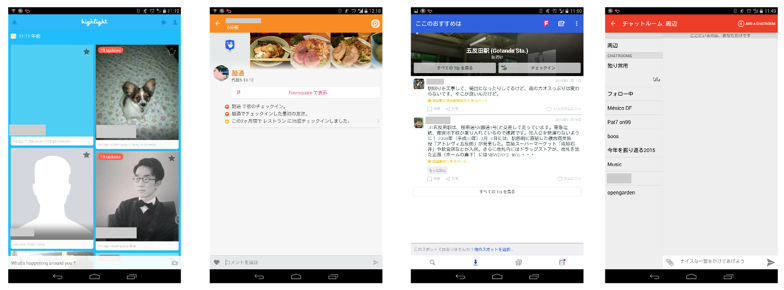
\includegraphics[width=1.0\linewidth]{img/contexts.eps}
    \end{center}
    \caption{Context-basedなサービス・アプリケーション}
    \label{fig:contexts}
\end{figure}


\section{今居るその場への情報共有手法}

人がその場に居合わせた他の人々へ情報を共有する、逆にその場に居合わせた人々から情報を取得する手法は、様々なものを検討することができる。

一般的なメールやSNSに依存したメッセージツールを使うのは、相手の連絡先をあらかじめ知っておく必要がある。
情報を共有したいが、個人間でなくその場を共有する多数の人間との共有を望んでいる場合、
個人の連絡先をまず共有するという手法は、プライバシーの面で安全とは言いがたい。
そのやりとりにはまず、個人間に十分な信頼が必要となる。
また、誰か一人が全体への共有を行うために連絡手法を呼びかけることもあるが、
誰もが偶然居合わせただけの状況では、集団を管理するのは難しいだろう。
その呼びかけも、誰もが自由に共有を行うプラットフォームとしては、手間の面で不便である。

その場を共有するための会場として設定する場合、NFCやWifiなどの機器を設置することによって共有のための空間を構築する手法は、
場に機器を設置する必要があり、何の設定もされていない場や、突発的な人間の集まりの場には対応することが難しくなる。

GPSセンサを使用した手法は、人々が携帯するモバイルデバイスには大抵の場合機能として含まれている上、
衛生から発信される電波を受信して測位を行うGPSには、場所を選ばないこともあり、一般的なセンサとして認識されている。
GPSの即位は広い距離範囲や平面的な距離測位において有効な効果を有するが、
測位の環境や電波状況などによって測位精度に影響が及ぶことにより、GPSは近距離での確実性を持った近接センサとは言い難い。

また、wifiによるアドホックな通信を行う手法では、昨今のモバイルデバイスの仕様上、
wifiのポートを通信中一つ専有することになるため、他の操作を阻害する恐れがある。
wifiのポートを2つ持つことが前提となるデバイスは、汎用的な手段としては選択し難い。

先行研究\cite{山本伶:2013-03-06}では、時限式で構造が変化するURLを共有することで
その場に居合わせた人間に対して情報を共有し、後からも変更、閲覧が可能な手法が提案されている。
本論文では、更に共有するためのキーワードも無く情報共有を行うことを可能にし、
あらかじめ名前の付いた場として設定されておらず、突発的な集団行動や普段の生活圏内の中でも情報共有が可能なサービスアプリケーションの提案を行う。


\section{近接情報取得手段としてのBluetooth無線技術}

Bluetooth\cite{bluetooth}は、GPSセンサと同じくモバイルデバイスに標準的に搭載されているモジュールである。
Bluetoothは電池持ちもいいし安価だし近接検出にとっても適してるよね

fireChat\cite{firechat}では、近接したデバイスとデバイスが、
インターネット回線に依存せずに通信しあうチャットコミュニケーション機能を有している。

Bluetoothを利用した、
ユーザが持つモバイルデバイス同士が近接したことを知るための
様々なアプリケーション\cite{すれちがったー}\cite{encountme}\cite{Monac}が存在する。



\section{デバイスによるアドホック通信}

\subsection{Bluetooth MANET}

MANETとは、Mobile Ad Hoc Networkの略称である。
MANET上のデバイスは上下左右、自由に移動可能な携帯性のあるデバイスである。
メッシュ・ネットワークの一つで、
通信拠点を介さず、デバイス同士でネットワークを構築して通信を行う。

アドホックネットワークとは、無線で接続可能な端末同士が専用の基地局やアクセスポイントを必要とせずに
通信を行う端末間のみで形成する無線ネットワークのことである。
通信にサーバを介さないため、インターネットに接続できない場所・状況でも相手ピアさえいれば通信が可能である。

そしてここで挙げるBluetooth MANETとは、Bluetoothによって築かれるMANETである。
Bluetoothの検出機能とペアリングを行って構築されるMANETであり、
一般的なAndroidモバイルデバイスに含まれるBluetoothは10mが検出範囲である。
この検出範囲は数珠つなぎのようにデバイスを連携させていくことによって検出範囲を広げていくことが可能で、この技術はホッピングと言われる。
先行研究ではBluetooth MANETによるものが提案されているが、
Bluetooth MANETはデバイスのペアリングが必要であり、ペアリングにはデバイス同士の認証が必要である。

また、Bluetooth4.0のプロトコルからは認証の必要が無い通信が可能となっている。
しかし、この通信でやりとり可能なデータ量はBluetoothによってペアリングしたデバイスや、インターネットに繋がっているデバイスに比べたら貧弱であり、
この手法が強力なのはインターネットが制限されている場合に限る。

本研究ではインターネットへの接続が制限されている状況を想定していないため、アドホックネットワークを用いず、
Bluetoothは近接するデバイスを検出する用途のみに利用する。

\chapter{設計}\label{chap:design}

本章ではその場に居合わせた人達の情報共有を可能にするサービスアプリケーションの設計について述べる。

\newpage

\section{アプリケーションの設計}

ここでは、その場に居合わせた人々が効率的に情報共有を行うためのアプリケーション、および周辺のシステムの設計について述べる。


\subsection{その場に居合わせていることへの保証}

ユーザが持っている近くに居るというコンテキストを判定するには、
第\ref{chap:background}章で述べたとおり、いくつかの手法が挙げられる。
確実にその場にいる人達との情報共有手法として、
Bluetoothによる近接デバイスの検出は適していると言える。
本アプリケーションでは、一般的なモバイルデバイスの持つBluetoothモジュールを利用した近接デバイス検出機能により、
その場に居合わせている人間の探索を実現する。


\subsection{情報の不揮発性}

本アプリケーションで共有された情報は、
発信地であるその場を離れても、受け取った人間が後で見返したり、
別の場所に共有することを可能とすることを目的としている。
そのためには、情報がその場限りで消えてしまうような揮発性を持ってはいけない。
情報の発信源である元のデバイスが近接する場所から離れても、
共有された情報は見られるように保存されるべきである。

アクティビティはアプリケーションがインストールされているデバイスに保管、
またはデータにアクセスできるよう保存され、
投稿された情報やメディアは後から見返せるようにする必要がある。

そのため、やりとりされる情報はMANETのような閉鎖的なネットワーク内でやりとりするのではなく、
全てWeb上に生成され、ブラウザ上から見られる方式が適していると考える。


\subsection{本人到達性とリンク可能性}

情報共有のサービスにおいては、
共有される情報とそれに結び付いた付加的な情報(発言者、時刻など)をどのように表現するかによって、
交わされる情報の内容が変化する。

例えば、発信者の本名および個人情報と結びついた情報ならば、
情報の内容は公共の場での発言と遜色のないものとなるだろう。
逆に匿名ならば、2ちゃんねる\cite{2ch}などに見る自由な発言内容が見られるだろう。

匿名性を測る指標として、本人を特定する本人到達性と、
表示されている投稿などが同一人物であるか判定するリンク可能性という、
2つの要素があると言われている。\cite{anon_terminology}

また、社会心理学の分野の研究\cite{diet}では、匿名性による社会的手がかりの減少から、
偏見やステレオタイプが避けられ、自己開示が促進されるメリットとともに、
共有された話題がテーマの場合は、情報に対する信頼度が十分に保たれるという結果が出ている。

\begin{figure}[h]
    \begin{center}
        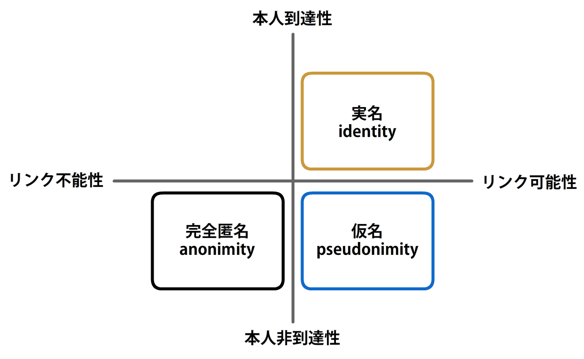
\includegraphics[width=0.8\linewidth]{img/anon.eps}
    \end{center}
    \caption{本人到達性とリンク可能性}
    \label{fig:anon}
\end{figure}

同じ場所に居合わせた見知らぬ人同士にとっては、情報開示に対するプライバシーの意識は敏感な問題である。
そのため、活発な情報開示を促進するために、匿名性を有するインターフェイスを提供する必要があると考える。

アプリケーションでは、リンク可能性を維持しながら、
本人到達性を減少させることで、仮名(pseudonym)によるサービスの設計を目指す。

\chapter{実装}\label{chap:implementation_1}

本章ではその場に居合わせた人達の情報共有を可能にするサービス・アプリケーションの設計と実装および機能について述べる。

\newpage

\section{そこにいる名無しさんの実装}

ここでは、アプリケーションの詳細な実装および有する機能について述べる。

\subsection{概要}

その場に居合わせた人達が情報共有をするためのサービス・アプリケーションのプロトタイプとして"そこにいる名無しさん"を実装した。
本アプリケーションは、人々が普段持ち歩いている一般的なモバイルデバイスが持つBluetoothモジュールと連携することにより、
その場に居合わせた同じアプリケーションを持った人達との情報共有を可能にし、また後から見返すことができる。

Androidのスマートフォンデバイスと内蔵されたBluetoothモジュールを使用したアプリケーションを試作した。

本アプリケーションは、2012年のつながり展、SFC OpenResearchForum2012においてプロトタイプが展示され、
来場者からのフィードバックを得た後、2013年に改良を加えたものである。


\subsection{システム構成}

本アプリケーションは、大きくAndroid\cite{AndroidDevelopers}デバイス、APIサーバ、データベースの3つに分かれる。
クライアントはアプリケーションを起動することでアプリケーションはAndroidデバイスに常駐し、付近のBluetooth端末を検出する。
検出した場合、APIサーバにMACアドレスを自分のMACアドレスと共に送信する。
APIサーバは、データベースにそれぞれのMACアドレスの存在を確認するとともに、存在するMACアドレスに紐付けられたアクティビティをデータベースから取得する。
最後に、APIサーバはアクティビティインターフェイスのためにデータを加工した状態でクライアントにデータを返信する。
クライアントは、以上の処理が完了したのち、アクティビティを閲覧することが可能となる。
また、自身のアクティビティを更新するのはどの時点でも可能である。

APIサーバは著者の自宅にあるUbuntu12.04、機能はNode.js0.10で記述した。
データベースはMySQL5.5を使用している。

\begin{figure}[h]
    \begin{center}
        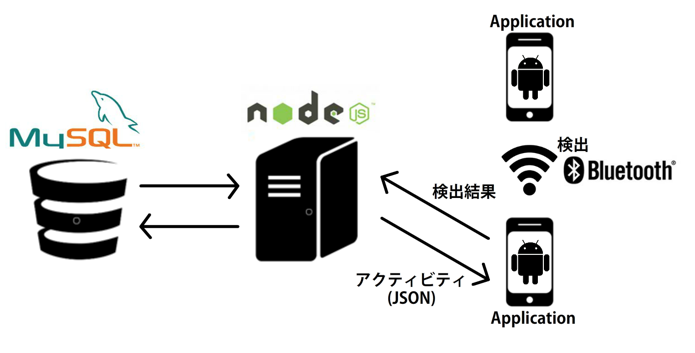
\includegraphics[width=1.0\linewidth]{img/servers.eps}
    \end{center}
    \caption{システム構成}
    \label{fig:servers}
\end{figure}

\newpage

\subsection{Androidアプリケーション}

プロトタイプを動作させる端末にはSamsung Galaxy NexusとASUS Nexus7 (2013)を使用した。
本アプリケーションで利用するBluetoothの機能は2.1のものであり、どちらとも機能要件を満たしている。
アプリケーションのソースコードはJavaで記述されている。

% 使用したデバイスに関するスペック表

\begin{table}[hb]
    \begin{center}
    \caption{Samsung Galaxy Nexus}

    \begin{tabular}{l|l}
        \hline
        OS & Android 4.0 \\
        画面サイズ & 4.7 インチ \\
        Bluetoothモジュール & Bluetooth 3.0 + EDR \\
        \hline
    \end{tabular}
    \end{center}
\end{table}

\begin{table}[hb]
    \begin{center}
        \caption{ASUS Nexus7 (2013)}

        \begin{tabular}{l|l}
            \hline
            OS & Android 4.3 \\
            画面サイズ & 7.02 インチ \\
            Bluetoothモジュール & Bluetooth 4.0 \\
            \hline
        \end{tabular}
    \end{center}
\end{table}

\newpage

\subsection{Bluetoothによるデバイス検出}

そこにいる名無しさんで実装に使用したAndroidデバイスでは、
周囲のBluetoothモジュールの検出にBluetooth2.1のプロトコルである検出機能を使用した。
検出を開始すると、およそ10秒間の間、周囲の検出可能なBluetoothモジュールを探索する。
検出可能なデバイスとは、あらかじめ自らを他のデバイスから検出可能な設定にしてあるBluetoothモジュールである。
Androidデバイスでは、デバイスのスキャンモードを検出可能(Discoverable)にすることで、行われる。

検出されたデバイスはBluetoothモジュールのMACアドレスが含まれるため、以降はこのMACアドレスをキーとしてデバイスを扱う。
これ以降に述べられる「MACアドレス」とは、全てBluetoothモジュールのMACアドレスのこととする。

一般的な携帯端末でのBluetooth検出効果範囲は10mである。検出の間、10m範囲内に検出可能なデバイスが含まれれば、検出結果に反映される。
10m以上に検出範囲を広げたい場合は、検出したデバイスが検出したデバイス、というようにデータを繋げていくことで実現可能となる。
これはホッピングと呼ばれ、Bluetooth MANETでは分散した機器が連携してデータをやりとりすることでホッピングを行うが、
本アプリケーションではBluetoothを近接デバイスの検出以上の機能は扱っていない。
ホッピングの機能は検出されたデバイスをサーバで管理することで、サーバ側での擬似的なホッピングを実装している。

検出可能なBluetoothモジュールは、探索の信号を受け取ると、レスポンスの信号を返すことにより、検出されることとなる。
また、Androidデバイスは、何も設定していない状態だと他のデバイスからの検出を無効にしている場合が多い。
今回使用した機種でもデフォルトでは無効の設定のため、アプリケーションはこの設定を監視し、常に有効にしている。


\subsection{サーバ・クライアントによる中央集権モデル}

Bluetoothを近接検出に利用した実装では、Bluetooth MANETを構築した分散モデルがある。
しかし、他のユーザーの投稿を扱う点で、それぞれのデバイスがデータを扱うのは、セキュリティ面で問題が残る。
本アプリケーションでは、後から投稿を閲覧する機能のために、サーバ・クライアントによる中央集権モデルを構築した。


\subsection{データベース・スキーマ}

データベースは、MySQLを使って実装されており、以下の3つのテーブルで構成される。

\begin{description}

\item{ユーザテーブル}

ユーザテーブルにはランダムに生成されたユニークなID情報をプライマリキーとして、
ユーザのBluetoothモジュールのMACアドレスが格納される。

\item{ユーザ検出テーブル}

ユーザ検出テーブルにはユーザが検出したMACアドレスのうち、
既にユーザテーブルに存在しているユーザ情報との結びつきが格納される。
格納される情報は、検出元のMACアドレス、検出されたMACアドレス、検出時間の3つである。

\item{ポストテーブル}

ポストテーブルには、ユーザが投稿したアクティビティが格納される。
格納される情報は投稿主であるユーザのMACアドレスと、
投稿の種類とその内容、投稿アクティビティのユニークIDである。
情報がメディアだった場合、blob形式で保存される。

\item{コメントテーブル}

コメントテーブルには、URL上から閲覧した人間がコメントを残した時にデータが格納される。
格納される情報は、コメント内容と、コメント先の投稿アクティビティが持つユニークなID、コメントが持つユニークなIDである。
コメントがメディアだった場合、blob形式で保存される。

\end{description}


\subsection{APIサーバ}

APIサーバは、クライアントからhttp通信で送られてきたデータを処理し、JSONフォーマットのデータ形式で返す役割を持っている。
APIサーバがインターフェイスとして持っているのは以下の3つである。

\begin{description}

\item{auth}

authは、クライアントがアプリケーション起動時にアクセスする場所で、ここではユーザの存在確認と認証を行う。
受け取ったユーザIDとMACアドレスをデータベースと照合し、ユーザの存在が確認できた場合はランダムな2つのユニーク色情報を生成して返す。
ここでMACアドレスのみを受け取った場合は、ランダムなユーザIDを生成後処理を行う。

\item{activity}

activityでは、ユーザIDと検出したMACアドレスの配列を受け取ってからMACアドレスがユーザテーブルに存在するか確認をとる。
存在していた場合はユーザ検出テーブルに検出元と検出されたユーザIDが現在時刻とともに挿入される。
検出されたユーザIDはユーザ検出テーブルから更に、検出されたユーザが10分以内に検出したユーザIDを取得する。
アプリケーションではこの操作をサーバ内での擬似的なホッピングと呼んでいる。
擬似ホッピングを3回行った後、一覧を重複のないユニークな一覧に整列した後、ポストテーブルから過去のアクティビティを取得する。
アクティビティは擬似ホッピングの際に計算された重複度の高い順に整列され、
ユーザの色ID情報を付加した後、JSONデータ形式でクライアントに返される。

\item{post}

postは、クライアントからユーザIDと投稿されたアクティビティを受け取る場所である。
受け取った情報は現在時刻と投稿固有のランダムなIDを付加された後、ポストテーブルに挿入される。

\item{get}

getでは、ユーザが投稿したアクティビティデータを扱う。
この場所だけは、JSONではなくHTMLデータを表示するビューが存在する。
get/[post ID]のようなURLでアクセスした時に、投稿されたアクティビティが単独で表示されるようになっている。
URLはアクティビティが投稿された際に生成される。
このURLは永続的なもので、URLを知っている人間はWebブラウザ上からアクティビティを閲覧することが可能である。
また、このページからはアクティビティへのコメント付加も可能である。

\item{comment}

commentでは、getの画面でPOSTメソッドによりコメントされたデータを扱う。
データはコメントテーブルに格納され、以降コメント対象となったアクティビティのページでコメントが閲覧できる。

\end{description}


\subsection{インターフェイス}

アプリケーションの初期画面インターフェイスは、チャットアプリケーションのタイムライン画面に似たデザインをしている。
アクティビティ画面、アクティビティの投稿画面はWebviewコンポーネントで表示しており、
インターフェイスに関わるソースコードはHTML, CSS, Javascriptによって記述されている。
サーバから受け取ったJSONデータはWebviewコンポーネントに受け渡され、Javascriptがデータを整形して表示する。

\subsection{アクティビティの投稿}

ユーザはアプリケーションの右上のボタンから、
自分のアクティビティを投稿することができる。
投稿されたアクティビティは、自分のデバイスを検出したユーザのアクティビティ画面と、
自分自身のアクティビティ画面に反映される。

またユーザはクライアントのアクティビティ投稿画面から、
文字だけでなくメディアファイルを共有することが可能である。

共有するメディアはアプリケーションサーバにアップロードされ、
アクティビティ画面にはメディアファイルへのリンクとして表示される。

\subsection{ブラウザからの投稿されたアクティビティの閲覧}

クライアントのアクティビティ画面から個別の投稿をタッチすると、ブラウザへのインテントが発生する。
インテントは、文字列の情報を指定したアプリケーションへ送信するAndroidの仕組みである。
ここでは、ブラウザに投稿されたアクティビティへのURLが受け渡され、
ユーザはブラウザから個別に投稿を閲覧することが可能となる。

\begin{figure}[hp]
  \begin{center}
    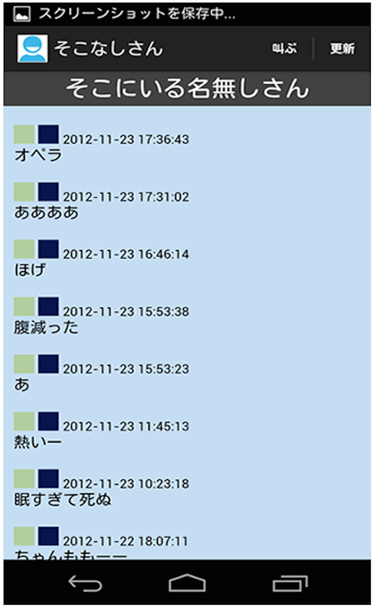
\includegraphics[width=0.5\linewidth]{img/v1_visual.eps}
  \end{center}
  \caption{インターフェイス}
  \label{fig:interface}
\end{figure}

\begin{figure}[t]
  \begin{center}
    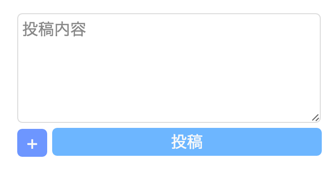
\includegraphics[width=0.5\linewidth]{img/post.eps}
  \end{center}
  \caption{投稿フォーム}
  \label{fig:post}
\end{figure}

\begin{figure}[t]
  \begin{center}
    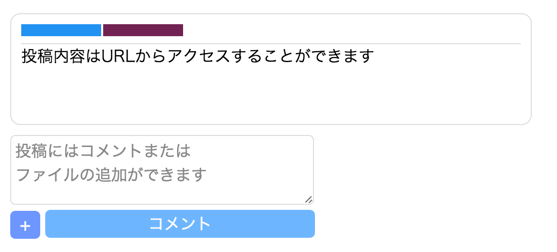
\includegraphics[width=0.8\linewidth]{img/get.eps}
  \end{center}
  \caption{ブラウザから見た投稿}
  \label{fig:get}
\end{figure}

\chapter{評価}\label{chap:hyoka}

本章ではアプリケーション「そこにいる名無しさん」の評価について述べる。

\newpage

\section{プロトタイプへの評価}

本アプリケーションは、当初チャット機能のみを有するプロトタイプを制作しており、
つながり展、ORF2012で展示を行った。

2013年には研究室内部の友人に操作してもらい、意見を集めている。

その中で、問題と改良のきっかけとなった代表的な意見を以下に挙げる。

\subsection{アプリケーション自体の話題拡散性について}

意見では、「このアプリケーション自体はバズらないのではないか」
バズるとは、ここではSNSやニュースサイトなどのインターネットのシーンで話題になることを言う。

プロトタイプのような、情報共有される範囲を空間位置的に制限した上に、
その場でコミュニケーションが完結するシステムでは、例え局所的に使われることがあっても
SNSやニュースサイトなどの公共のシーンで気づかれることはない。
そのため、アプリケーションが有用であっても、広まるのは非常に困難だろうという指摘があった。

改良版では情報共有を行った後の閲覧と編集に重点を置き、情報共有のためのWebインターフェイスを追加した。

\subsection{発言内容の出現・消滅タイミングによる本人到達性について}

プロトタイプでは、検出したデバイスの判定から逐次、アクティビティ画面を完全に更新していた。
それにより、現在どの発言者が近くにいて、どの発言者が離れたか推察できてしまう可能性の問題があった。

そのため、アクティビティ画面では投稿の順序や距離による順序を気にしないよう、
ユーザごとに独自に積み重なってゆくインターフェイスへ改良した。

\chapter{ユーザ情報の偏在化}\label{chap:implementation_2}

ここでは、そこにいる名無しさんを補助する目的で作られたユーザ管理システムについて述べる。

\newpage

\section{概要}

そこにいる名無しさんのシステムでは、近くにユーザ数が確保できない限り、
アクティビティの内容が活性化しないという問題があった。

近年では人々が持ち歩くモバイルデバイスは、スマートフォンだけに留まらず、様々なデバイスを持ち歩くようになってきている。
そのなかでも、Bluetoothモジュールは大抵のモバイルデバイスに付属しており、
Bluetooth近接検出では一人の人間に対して復数のデバイスを検出することもままある。

本アプリケーションは、本論文の実装物であるそこにいる名無しさんの効果を高めるため、
ユーザが持つモバイルデバイスとは別に、スレイヴとして別端末も同じユーザとみなす効果をもたらすための
アプリケーションである。


\newpage

\section{設計}

\subsection{デバイスの検出とユーザが結びつく確実性}

ここまでは、ユーザと紐付いたデバイスが検出されたならば、そこにユーザが居るという前提に立って述べてきた。
しかしユーザが持っているデバイスは一つとは限らず、検出されるのが紐付いたデバイスであるとは限らない。
例えば分厚い鞄に入ったデバイスは、電波状況のために検出から逸れることもままある。
そんな時に予備としてユーザと紐付いたデバイスがあれば、周囲のアプリケーションからは同じ効果が得られる。



\newpage

\section{実装}

\subsection{システム構成}

本システムは、そこにいる名無しさんと同じく、Androidアプリケーション、APIサーバ、データベースの3つで構成されている。

AndroidアプリケーションはJava、APIサーバはNode.js0.10、以降のシステムはそこにいる名無しさんと共有している。

\subsection{APIインターフェイス}

\begin{description}

  \item{adduser}

adduserからは、既に登録されたMACアドレスとユーザID、新たに追加するMACアドレスを受け付ける。
サーバは、既に登録されたMACアドレスからユーザ情報をデータベースから取り寄せ、
新たに追加するMACアドレスをスレイヴとして登録する。

\end{description}

\subsection{アプリケーション}

アプリケーションはそこにいる名無しさんと同じくBluetooth2.1プロトコルの検出機能を利用し、
周囲のデバイスを検出する。このとき、検出対象になるのはアプリケーションが入っているモバイルデバイスと
既にペアリングされているデバイスのみである。

アプリケーションはペアリングされているデバイスをユーザのスレイヴデバイスとみなし、
APIサーバに自らのMACアドレスと、スレイヴとみなすデバイスのMACアドレスを送信する。

これにより、以降はそこにいる名無しさん側でも、スレイヴデバイスをユーザの持つモバイルデバイスとみなすようになる。


%画像が入る

\chapter{応用例}\label{chap:application}

本章では、本論文で提案されるアプリケーションを使った応用例について述べる。

\newpage

\section{同じ目的を持った人間の集まり}

例えば、イベント会場やライブ会場などは、同じ場所と状況をその場に居る人々が共有していることになる。
そのまま過ごしていれば、お互い名前も連絡先も知らない人同士ですれ違って終わってしまうが、
これが例えば見知った人ばかりならば状況に対する情報共有は、それが会話によるものであったり、
モバイルデバイスのメッセージツールであったりしながら活発になることだろう。
この2つの状況の違いをツールで埋めることで、その場に対する情報共有の勢いは最大化されることができる。

\section{偶然発生した状況に居合わせた場合}

先行研究では、情報を共有する場として設定されている場面は、あらかじめ名前の付けられたものである。
しかし例えば電車の事故などで電車内に閉じ込められた状況なども、その場の人間とは名前も連絡先も知らない人同士であり、
なおかつその場に対する情報を求めることの多い場面である。
このような突発的な人間の集合による状況の共有では、情報を管理しつつ共有するようなことは難しい。

モバイルデバイスを持っていればその場の情報にアクセス可能であるというのは、
人間の集まりを取り仕切って情報を管理する人が居ないような状況では強力であると言える。



% \section{イラクでのデモ、中国でのデモの例}

\chapter{関連研究}\label{chap:related}

本章では、関連研究、及び本論文に関連する先行サービスについて紹介する。
初めに近接情報の検出に関するもの、
続いてその場の情報共有に関するものを紹介する。
最後にこれらを踏まえた本研究との比較について述べる。

\newpage

\section{近接情報の検出に関するもの}

はじめに、Context-basedなサービスに関する先行サービスおよび関連研究について紹介する。

Google Latitude\cite{latitude}は、Googleが提供するGoogle Mapsの機能として使用することのできた位置情報サービス。
Google Maps上で有効にしておくと、友達や家族など、共有を設定したユーザーと互いの現在位置をGoogle Maps上で共有できる。
2013年8月9日にサービスを終了している。

FourSquare\cite{foursquare}は、GPSによる居場所の特定とチェックインと呼ばれるユーザの来訪履歴を組み合わせたサービス・アプリケーション。
サービス上で登録しておいた友人が近くの登録された施設にチェックインをすると、情報をプッシュ通知を受け取ることが可能になる。
また、近くに友人が来訪した履歴のある施設があると、これもプッシュ通知として表示される。

\cite{槙島量:2010-03-08}は、リアルタイム性のある地域情報をデバイスに対してPush通知するシステムを提案した。
本提案では、地域を50mの矩形に分割することで、その地域の情報を通知できる他、
同矩形範囲内のユーザからも情報を引き出すことで、ユーザ同士のリアルタイムなコミュニケーションを実現している。

Bluetoothの近接検出に関して、Davidrajuh\cite{Davidrajuh:2009:EPB:1523492.1523495}らは、
マスタデバイスとPico-net上の2つのスレーブデバイスでプロトタイプを作り、
大きなサイズの教室内でのBluetooth無線技術によるScatter-net環境が有用であることを示した。

DroidSensor/すれちがったー\cite{すれちがったー}は、2009年から2010年にかけて配布されていたBluetoothとTwitterを使った、すれちがい通信アプリケーション。
すれちがったーをインストールしたデバイスが同じくインストールされた他のデバイスとすれちがうと相手のtwitter IDを呟く。
他のデバイスがすれちがったBluetoothデバイスとすれちがうと、以前にそのデバイスとすれちがった相手のtwitter IDを呟く。
どのデバイスとすれちがったかをトラッキングすることで、twitter IDを持つ本人を特定できてしまうというセキュリティの問題が議論された。


% 画像

\section{その場の情報共有に関するもの}

\subsection{Firechat}

Firechat\cite{firechat}は、OpenGardenによるApple iOSとGoogle Android向けのチャットコミュニケーションアプリ。

登録された人間同士のチャット機能の他に「周辺」というチャットルーム機能を持つ。
モバイルデバイス同士がメッシュネットワークを築くことによりインターネット接続が無くてもチャット通信が可能。
メッシュネットワークを数珠つなぎのように延ばすことで、最大70mまでのホッピングを可能としている。
Bluetooth検出のホッピングにより、最大で70mまでのデバイス検出を可能としている。

また、同様の機能を持ったアプリケーションに、2007年にはBluetoothを利用して近場のデバイス同士でチャットを行うBlueeee!\cite{Blueeee}がある。


\subsection{ライブ情報共有のためのすれちがい通信アプリ}

藤田ら、\cite{藤田大樹:2012-09-04}\cite{藤田大樹:2013-08-20}\cite{藤田大樹:2013-03-06}は、
iOS上で動作する,アドホックネットワークを用いて周囲とライブ情報を共有するためのプロトタイプLNSを実装した。
本研究はすれ違い通信\cite{菊池大輝:2012-09-04}によってライブ情報を適切な範囲に対して拡散させるためのシステムを
提案しており、共有するメッセージの有効時間とホップ数を適切に設定することで、メッセージの到達可能範囲を
発信者の近隣のみに限定した上、有効時間が切れたメッセージを自動で削除することが可能だと述べている。

\begin{figure}[h]
  \begin{center}
    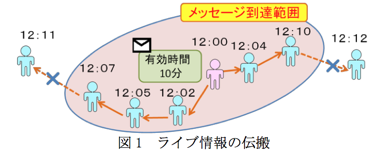
\includegraphics[width=0.5\linewidth]{img/live.eps}
  \end{center}
  \caption{システム構成}
  \label{fig:live}
\end{figure}

\subsection{Sonoba.org}

山本らは、情報をその場に居る人達に共有する手法としてSonoba.org\cite{山本伶:2013-03-06}を提案した。
本研究では、たまたま居合わせただけのような、
よく知らない相手とのその場限りの関係においてもデジタルな情報の共有をする方法として、
時限URLを用いた手法を提案し、Sonoba.orgとして実装した。
この提案では、誰もが普段持ち歩いているモバイルデバイスから共有する情報にアクセスするため、
覚えやすい文字列と、時限式で消去されるURLによる共有手法を使うことにより、その場限りの共有手法を実現している。

\begin{figure}[h]
  \begin{center}
    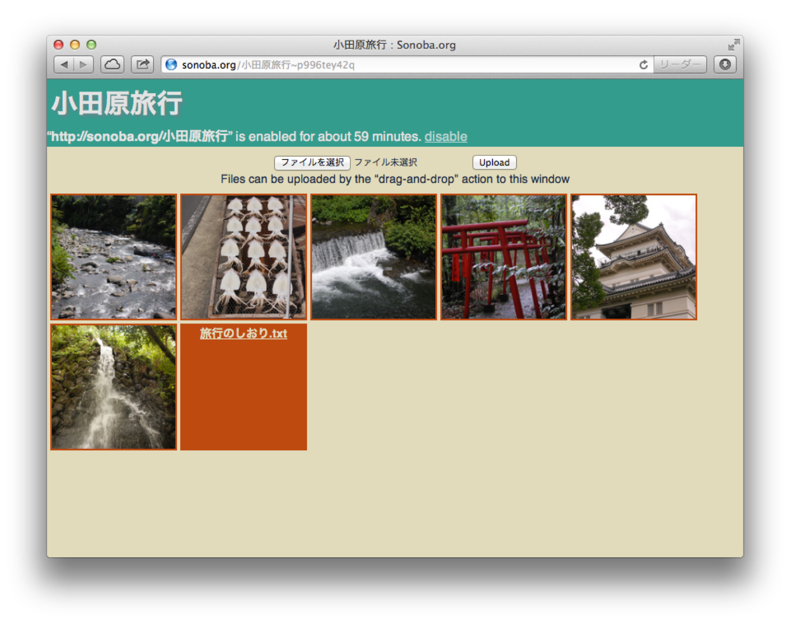
\includegraphics[width=0.7\linewidth]{img/sonoba.eps}
  \end{center}
  \caption{システム構成}
  \label{fig:sonoba}
\end{figure}

\subsection{Encore}

Adityaらは、イベント参加者の間でコミュニケーションと共有を可能にするアプリケーション、Encoreを提案した。\cite{Aditya:2014:EPC:2594368.2594374}
2つのデバイスがBluetoothの無線範囲内に存在するとき、デバイスは共有鍵を生成した上で、Bluetooth無線による通信を行う。
また、このシステムの共有鍵については、Manweilerら\cite{Manweiler:2009:SET:1653662.1653692}によれば、
デバイス感の共有鍵の交換によって、悪意のある接続から守ることが可能であると述べている。



\section{関連研究と本研究との比較}

本研究は、Sonoba.org\cite{山本伶:2013-03-06}と、近接情報の検出の文脈を受け継いでいる。
その場に居合わせた人間同士で自動的に共有のための場が作られる手法として、
近接しているというコンテキストを利用するのは強力であると言える。
それに加え、Webを介した情報共有の利便性と、情報の継続性も持つことができた。

URLの共有によってWeb上での情報共有を図る手段に比べると、
どうしてもアプリケーションのインストールという手間がある。

また、Bluetoothにおけるセキュリティとプライバシーの問題を隠匿して吸収するために、
本システムではほとんどの情報処理をサーバ側で担っている。
この構造は、ユーザが増加した時にサーバ管理のコスト増大があることは明確であり、
より低コストな構造の検討が求められる。

\chapter{考察と今後の課題、議論}
\label{chap:discussion}

本章では、本論文で提案したアプリケーションの有用性についての考察をおこなう。
本アプリケーションの実装に関する議論と考察を述べる。


\newpage

\section{プライバシーとセキュリティ}

\subsection{アクティビティのURLについて}

アクティビティに割り当てられるURLは仕様上、誰でも閲覧することが出来る。
URLの文字列は複雑なハッシュ値を持っており、
知らなければ偶然辿り着くようにはなっていない。
しかし、意思が介在すれば誰でも見られる場所にURLを共有することも可能なので、
不特定多数が閲覧するにはセンシティブな情報共有には向いていない。
そのため、投稿の揮発性を低減させた分、
投稿の内容が場所や状況に特化したものになるかどうかの議論がある。


\subsection{無線検出におけるプライバシーとセキュリティ}

Bluetoothによるデバイス検出機能を利用したサービスアプリケーションには、
プライバシーの問題が多く取り沙汰されている。
所持するデバイスを常に検出可能な状態にしておくのは、
検出されたMACアドレスとデバイスを結びつけ、本人到達性を増加させるおそれがある。
デバイスを繰り返し検出し続けることで人の位置と検出されたデバイス名から、
BluetoothデバイスのMACアドレスとデバイスの持ち主の結びつきを類推または特定することが可能である。
また、MACアドレスの持つ前半6つの文字はベンダー固有のものであり、
検出されたMACアドレスとアプリケーションで共有された情報の繋がりをユーザが閲覧できる状態にしておくと、
持っているデバイスとMACアドレスから、発言者の類推が可能になってしまう。
これも本人到達性を増加させる原因となる。
本アプリケーションの実装では、検出したMACアドレスはサーバに送信する以外の操作を行っておらず、
また、インターフェイスもMACアドレスとの結びつきを類推することがないようにしている。
今回の実装で扱った情報では問題は無いが、今後扱う情報がより多く、プライバシーに関わる内容が扱われる場合、
プライバシーに配慮した仕組みが必要になってくるだろう。


\section{Bluetoothの特性に関して}

\subsection{限られた効果範囲}

Bluetoothの10mという効果範囲は、
局所的な使用としては適しているものの、
使い始めの際には同じアプリケーションを持ったデバイスが周囲に存在しない限り、
効果を発揮することが出来ない。
ホッピングすることにより効果範囲を広げることが可能となるが、
ホッピングのための中継地点としても、ユーザが必要になってくる。
先行サービスは、人が密集している状況で示し合わせて使われるという
広まり方をしたものがあるが、そういった特殊な状況だけでなく、
普段の状況からでも利用ができるような仕組みが求められる。

\subsection{バージョン間の仕様の違い}

Bluetoothコア仕様では、バージョン4.0以降、
Bluetooth Low Energy(Bluetooth LE)などの異なる種類のBluetoothプロトコルが定義されている。
そのため今回の実装に使われているBluetooth2.1のプロトコルはクラシックBluetoothと呼ばれている。
Bluetooth LEは従来のクラシックBluetoothよりも電池消費の面で優れており、
常時使用するアプリケーションにはこちらの方が適していると言われている。
このBluetooth LEとクラシックBluetoothは検出方法の仕様に違いがあり、
今後実装の展開によっては、クラシックBluetoothの仕様を切り離すことも考えられる。
しかしその場合、クラシックBluetoothしか持たないデバイスを切り離すことにもなる。
このことと、上記に挙げたデバイス検出の問題は、考慮されるべきことだと思われる。

\subsection{リアルタイムな検出による問題}

今までの近接検出では結局、示し合わせて同じタイミングで使わなくては効果が無い
近接検出のより強力な使用法が求められる

\chapter{結論}\label{chap:conclusion}

本章では、本論文で提案されたアプリケーションの成果を確認したのち、
展望について述べ、本論文を統括する。

\newpage

\section{研究成果}

本論文では、同じコンテキストを持った人同士を繋ぐサービスについて紹介し、
同じ場所や状況を共有する人々の間で行う情報共有についての問題を整理した上で、
その場への情報共有手法としてBluetoothとモバイルデバイス、Webの連携を行ったサービスを提案した。
また、提案からプロトタイプ「そこにいる名無しさん」を設計・実装し、
そのフィードバックから改良を重ねたアプリケーションから共有手法の有効性の考察を行った。

\section{展望}

「そこにいる名無しさん」の設計では、その場で共有された情報をWeb上で閲覧できる仕組みを構築した。
偶然その場に居合わせた人同士がデジタルな情報を共有する手法は、
情報の信頼性の向上と、空間的に適切な有効範囲を探っていく必要がある。
また、今回はBluetooth2.1のプロトコルを利用したシステムの提案を行ったが、
Bluetooth LEによる、より電池消費が少なく柔軟な検出方法も含め、
より適切な近接情報の検出手法を検討していく。

Web上からアクセスできる情報として、現在の実装はアクティビティごとのページ生成となっているが、
更に状況の空気感と言えるものも閲覧できるように、まとめのようなページも生成できるようにできるとなお良いと言える。
そのためにも、アクティビティの中に場の空気を感じられるようなインターフェイスを探っていく必要もある。


\section{結論}

近接デバイスの検出手段としてのBluetoothは、
一般的なモバイルデバイスのモジュールの中でも安価で手に入り、
電池の消費量の面でも非常に優秀なセンサとして活用することができる。
このモジュールの利用とWebの組み合わせによって、どんな状況でもその場に居合わせたというコンテキストを証明することが可能となった。

近接するモバイルデバイスの検出という面でBluetoothは強力な効果を持っており、
これからも、ユーザのコンテキストを読み取る手段としてのBluetoothモジュールはその有効性を示していくだろう。

また、そこからモバイルデバイスに含まれる機能と組み合わせることで、
その場への情報共有手法としてのモバイルデバイスの活用はより活発に、よりユーザの目的に沿った形で実現されると思われる。

情報共有手法としてのアプリケーションである本提案により、
近接情報の検出をベースにした同じ場に偶然居合わせた人同士の共有手法と、
その場を離れても情報の共有を継続できる手法を提示できたと考えている。


\chapter{本研究に関する発表}\label{chap:publication}

\section{展示会}

\begin{itemize}

\item つながり展 (2012年9月13日〜15日
慶應義塾大学日吉キャンパス 来往舎2F ギャラリー \
展示会、主催:慶應義塾大学 SFC インタラクションデザインラボ)

\item SFC OpenResearchForum2012 (2012年11月22日〜23日
東京ミッドタウンホール \
カンファレンス、主催:慶應義塾大学SFC研究所)

\item SFC OpenResearchForum2013 (2013年11月22日〜23日
東京ミッドタウンホール \
カンファレンス、主催:慶應義塾大学SFC研究所)

\end{itemize}


\begin{acknowledgment}

修士課程の2年間、研究をご指導いただいてきた慶應義塾大学環境情報学部の増井俊之教授に深く感謝致します。
また、本研究の副査としてご意見、ご助言を頂きました徳田教授、高汐准教授に感謝致します。
中間考査の際には、CIの様々な教授陣の方々からご意見、アドバイスをいただきました。

2年間のIDP(インタラクションデザインプロジェクト)に在籍していた間、メンバーたちと多くの議論をすることができました。
メンバーである臼杵壮也くん、馬場匠見くん、田中優くん、桜井雄介くん、中園翔くんには、研究だけでなく
日々の活動や議論の場でも支えられてきたことを感謝いたします。
中園翔くんには、学業の面でも多大な貢献をしてくださったことを感謝いたします。

大学院生の活動であるIDPだけでなく、学部研究会のメンバーの方々とも活発な議論をさせていただくことが多く、
日々の研究活動の支えになっていただきました。
本研究のサーバサイド実装の土台は、学部研究会メンバーであった片倉弘貴くんのテンプレートを参考にさせていただきました。

修士論文執筆にあたっては、学部時代の先輩にあたる黒井さんと山本伶さんが作ったテンプレート、
そしてさらに馬場匠見くんが改良を重ねてくれたものをお借りしています。

本論文における研究の前進は、学部時代に所属していた安村研究室の頃から続けられてきたものです。
安村研究室の皆様、および安村先生には、様々なアドバイスや意見をいただいたことを感謝いたします。
また、研究の文脈であるIDPのOBの方々の研究活動からも、多くのことを学ばさせていただきました。

最後に、私の学生活動並びに大学院への進学を応援し、支えてくれた家族と友人の方々に、深く感謝いたします。

\begin{flushright}
2015年1月 慶應義塾大学政策・メディア研究科 修士2年

郡山 隼人
\end{flushright}



\end{acknowledgment}
  % 謝辞。要独自コマンド、include先参照のこと
\begin{bib}[100]
    % BibTeXを使う場合
    \bibliography{main}

    %\begin{thebibliography}{#1}
    %
    %  \bibitem{参照用名称}
    %    著者名:
    %    \newblock 文献名,
    %    \newblock 書誌情報,出版年.
    %
    % \bibitem{hoge09}
    %   ほげ山太郎,ほげ山次郎:
    %   \newblock ほげほげ理論のHCI分野への応用,
    %   \newblock ほげほげ学会論文誌,Vol.31,No.3,pp.194-201,2009.
    %
    % \bibitem{hoge08}
    %   Taro Hogeyama, Jiro Hogeyama:
    %   \newblock The Theory of Hoge,
    %   \newblock {\it The Proceedings of The Hoge Society}, 2008.
    %
    %\end{thebibliography}

\end{bib}
  % 参考文献。要独自コマンド、include先参照のこと
%\appendix
%\chapter{付録の例}

付録を無理矢理出力させるため、てきとうなことを書く。

\section{ほげ}

コマンドは本文と一緒。

\section{ほげほげ}

本文と一緒。

\subsection{ふーふー}

本文と一緒。
    % 付録

\end{document}
